\documentclass[12pt]{iopart}
\usepackage{iopams}  
\usepackage{graphicx}
\usepackage{subfig}
\setlength\parindent{0pt}
\setlength{\parskip}{13pt} %found this single-line pt value using \the\baselineskip
\begin{document}

\title[]{Cauchy Evolution of Asymptotically AdS Spacetimes with No Symmetries}

\author{Hans Bantilan$^1$, Pau Figueras$^1$, Lorenzo Rossi$^1$}
\address{$^1$ School of Mathematical Sciences, Queen Mary University of
  London, \\ Mile End Road, London E1 4NS, United Kingdom}
\ead{l.rossi@qmul.ac.uk}

\begin{abstract}
We present the first proof-of-principle Cauchy evolutions of asymptotically AdS spacetimes with no symmetries.
We use a numerical scheme that is based on the generalized harmonic form of the Einstein equations expressed in Cartesian coordinates.
For this first study, we perform 3+1 simulations of four dimensional spacetimes with a negative cosmological constant, using initial data sourced by a massless scalar field.
We demonstrate stable and convergent Cauchy evolution of horizonless data, as well as data that undergoes gravitational collapse.
The main difficulty in removing all symmetry restrictions in this setting is to find a generalized harmonic gauge choice that is consistent with the AdS boundary conditions.
We explicitly write down the gauge choice that achieves this in terms of a specific choice of generalized harmonic source functions.
These preliminary results are a direct precursor to important specialized studies of AdS dynamics with no symmetry assumptions, most notably of gravitational collapse, and of the superradiant instability.
\end{abstract}


\noindent{Keywords}: AdS, generalized harmonic, 3+1, superradiance, gravitational collapse

% Uncomment for Submitted to journal title message
%\submitto{\JPA}
%
% Uncomment if a separate title page is required
%\maketitle
% 
% For two-column output uncomment the next line and choose [10pt] rather than [12pt] in the \documentclass declaration
%\ioptwocol




\section{Introduction}

In an unprecedented way, the simulation of asymptotically anti-de Sitter (AdS) spacetimes has opened up the field of numerical relativity to the study of phenomena in areas beyond General Relativity (GR). 
At the heart of this push to understand AdS is a deep mathematical connection between gravity in AdS to certain conformal field theories (CFT), now known as the AdS/CFT correspondence~\cite{Maldacena:1997re,Gubser:1998bc,Witten:1998qj}. 
Through this connection, the study of AdS spacetimes has become immediately relevant to fundamental questions in many areas in physics, such as fluid dynamics [cite], relativistic heavy ion collisions [cite], and superconductivity [cite].
See, for example, [cite] for excellent reviews. 

The reason the study of AdS is crucial for our understanding of these phenomena is that AdS/CFT provides an important --and in most cases the only-- window into the real-time dynamics of quantum field theories far from equilibrium. 
The dynamical far-from-equilibrium regime is precisely the one that is least explored and understood, and the one that has the best chance of making contact with experiment.
Within GR, the dynamics of AdS provides a detailed look at how the Einstein equations behave in the fully non-linear regime and with non-trivial boundary conditions.
This has led to important progress in our understanding fundamental phenomena in gravity, such as gravitational collapse, black hole collisions, and superradiance. 

Our current understanding of AdS, however, remains limited. 
This is due to several reasons.
First, evolution in AdS is notoriously hard, in part because it is an initial boundary value problem whose systematic study is still in its infancy. 
Cauchy evolution in AdS requires data to be prescribed not only at an initial space-like hypersurface, but also at spatial and null infinity which constitute the time-like boundary of an asymptotically AdS spacetime.
Second, the most interesting phenomena involve spacetimes that have very little or no symmetry, making these evolutions beyond the reach of most numerical codes. 
Third, for many of these phenomena, there is a variety of physical scales that must be adequately resolved to capture the correct physics.

The main purpose of this article is to present the first proof-of-principle Cauchy evolution of asymptotically AdS spacetimes that has been achieved with no symmetry assumptions.
The results presented here are based on a code that solves the Einstein equations for asymptotically AdS spacetimes with a generalized harmonic evolution scheme, with adaptive mesh refinement capabilities. 
This code is the next step in an ongoing program initiated in \cite{Bantilan:2017kok} that uses Cartesian coordinates in global AdS, now enabled with a breakthrough set of generalized harmonic source functions that is crucial in successfully stabilizing evolution in AdS with no symmetries.

This article is organized as follows. 
In Section~\ref{sec:setup} we describe the setup, and in Section~\ref{sec:numerical_scheme} we outline the generalized harmonic scheme that we use in our simulations.
In Section~\ref{sec:gauge_choice} we explicitly write down our gauge choice in terms of a specific choice of generalized harmonic source functions that stabilizes these evolutions with no symmetry.
Section~\ref{sec:results} contains preliminary results from this new code, and we conclude with a discussion in Section~\ref{sec:Discussion}.



\section{Setup}\label{sec:setup}

The dynamics of gravity with a cosmological constant $\Lambda$ in four dimensions coupled to a massless scalar field $\varphi$ can be described by the following action
\begin{equation}\label{eqn:action}
S = \int d^4 x \sqrt{-g} \left( \frac{1}{16\pi} \left( R - 2\Lambda \right) - g^{\alpha\beta} \partial_\alpha \varphi \partial_\beta \varphi \right),
\end{equation}
where $R$ is the Ricci scalar of the metric $g_{\mu\nu}$ with determinant $g$.
Here, we use geometric units where Newton's constant $G$ and the speed of light $c$ are set to 1.
The variation of the action \eref{eqn:action} with respect to $g_{\mu\nu}$ and $\varphi$ gives the equations of motion
\begin{eqnarray}\label{eqn:eoms1}
R_{\mu\nu} - \frac{1}{2} R g_{\mu\nu} + \Lambda g_{\mu\nu} = 8\pi \left( \partial_\mu \varphi \partial_\nu \varphi - g_{\mu\nu} \frac{1}{2} g^{\alpha\beta} \partial_{\alpha} \varphi \partial_{\beta} \varphi \right),
\end{eqnarray}
\begin{equation}\label{eqn:eoms2}
g^{\alpha\beta} \nabla_{\alpha} \nabla_{\beta} \varphi = 0.
\end{equation}
The metric of AdS$_4$ is the maximally symmetric vacuum (i.e. $\varphi=0$) solution of \eref{eqn:eoms1},\eref{eqn:eoms2} in four dimensions.
In terms of global coordinates $x^\mu=(t,r,\theta,\phi)$ that cover the whole spacetime, the metric of AdS$_4$ can be expressed as
\begin{equation}\label{eqn:ads4}
\hat{g}_{\mu\nu} dx^\mu dx^\nu = \left( -(1+r^2/L^2) dt^2 + (1+r^2/L^2)^{-1} dr^2 +r^2 d{\Omega_2}^2 \right), \nonumber
\end{equation}
with a characteristic length scale $L$ that is related to the cosmological constant by $\Lambda = - 3/L^2$, and $d{\Omega_2}^2 = d\theta^2 + \sin^2\theta d\phi^2$ is the metric of the round 2-sphere.

First, we compactify $r=2\rho/(1-\rho^2/\ell^2)$ to include the boundary at $r \rightarrow \infty$ as part of the spacetime at $\rho=\ell$.
We hereafter set to $\ell=1$ without loss of generality, so that the AdS boundary is $\rho=1$.
Defining a convenient function $\hat{f}(\rho) = (1-\rho^2)^2+4\rho^2/L^2$, this compactification brings the metric of AdS$_4$ into the form
\begin{equation}\label{eqn:ads4_compact}
\hat{g} = \frac{1}{(1-\rho^2)^2} \left( -\hat{f}(\rho) dt^2 + 4(1+\rho^2)^2 \hat{f}(\rho)^{-1} d\rho^2 + 4\rho^2 d{\Omega_2}^2 \right). \nonumber
\end{equation}

Second, we define Cartesian coordinates $x=\rho\cos\theta$, $y=\rho\sin\theta\cos\phi$, $z=\rho\sin\theta\sin\phi$ where $\rho=\sqrt{x^2+y^2+z^2}$, in order to bypass the severe restriction on time step size at the origin $\rho=0$ of a grid in polar coordinates. 
This brings the metric of AdS$_4$ into its final form
\begin{eqnarray}\label{eqn:ads4_final}
\hat{g}=&\frac{1}{\left(1-\rho^2\right)^2 }\left( -dt^2 \hat{f}(\rho) +4\rho^{-2}\hat{f}^{-1}(\rho) \left(1+\rho^2\right)^2 (x dx + y dy + z dz)^2 \right. \nonumber \\
&+\frac{4}{\rho^2} \left[\left(-2 x y\right) dx dy + \left(- 2 y z\right) dy dz + \left(- 2 x z\right) dx dz \right. \nonumber \\
&\left. \left. + \left(y^2+z^2\right) dx^2 + \left(x^2+z^2\right) dy^2 + \left(x^2+y^2\right) dz^2 \right] \right),
\end{eqnarray}



\section{Numerical Scheme}\label{sec:numerical_scheme}

We solve the Einstein equations in generalized harmonic form~\cite{Pretorius:2004jg} with constraint damping, for asymptotically AdS spacetimes~\cite{Bantilan:2012vu}.
We discretize the resulting PDEs with second order finite differences, and integrate in time using an iterative Newton-Gauss-Seidel relaxation procedure. 
We use the PAMR/AMRD libraries \cite{PAMR} for running these simulations in parallel on Linux computing clusters and for adaptive mesh refinement support.
We obtain initial data using a multigrid algorithm built into the PAMR/AMRD libraries.
The numerical grid is in $(t,x,y,z)$ with $t \in [0,t_{max}]$, $x \in [-1,1]$, $y \in [-1,1], z \in [-1,1]$.
The typical grid resolution gives $N_x=N_y=N_z=257$ points in each of the Cartesian directions, with equal grid spacings $\Delta x = \Delta y = \Delta z$.
We use a typical Courant factor of $\delta \equiv \Delta t / \Delta x = 0.2$.

We search for apparent horizons (AH) using a flow method, and use the excision method to evolve black hole spacetimes, thereby removing geometric singularities from the computational domain.
At the excision surface, the usual equations of motion are solved using one-sided stencils. 
Kreiss-Oliger dissipation~\cite{kreiss1973methods} is essential to damp unphysical high-frequency noise that arise at such grid boundaries, and we use a typical dissipation parameter of $\epsilon=0.35$.

We set Dirichlet boundary conditions at the AdS boundary $\rho=1$ for all evolved variables. 
The simulations described here are performed in Cartesian coordinates $x,y,z$ in terms of which $\rho^2=x^2+y^2+z^2$, so the AdS boundary generally does not lie on a Cartesian grid point. 
For any given evolved variable, we thus take its Dirichlet boundary condition at $\rho=1$ and its values at points further to the interior $\rho<1$, and use these to set its value at grid points that are at most one grid point away from $\rho=1$ by linear interpolation.

The evolved variables $\bar{g}_{\mu\nu}$ are constructed out of the full metric $g_{\mu\nu}$ and the pure AdS metric $\hat{g}_{\mu\nu}$ by $g_{\mu\nu} = \hat{g}_{\mu\nu} + \bar{g}_{\mu\nu}$. 
Similarly, the evolved source function variables $\bar{H}_\mu$ are constructed out of the full generalized harmonic source functions $H_\mu$ and the values they take on in pure AdS $\hat{H}_\mu$ by $H_\mu = \hat{H}_\mu + (1-\rho^2) \bar{H}_\mu$.
The evolved scalar field variable $\bar{\varphi}$ is constructed out of a real scalar field $\varphi$ by
$\varphi = (1-\rho^2)^2 \bar{\varphi}$.
By construction, the evolved variables $\bar{g}_{\mu \nu}$, $\bar{H}_{\mu}$, $\bar{\varphi}$ all fall off linearly in $(1-\rho)$ near the AdS boundary $\rho=1$. 



\section{Gauge Choice}\label{sec:gauge_choice}

Here we sketch the procedure for finding the generalized harmonic gauge choice that achieves stable Cauchy 3+1 evolution in for asymptotically AdS$_4$ spacetimes.
For a more detailed discussion in a simpler context with more symmetry, see~\cite{Bantilan:2012vu}. 
The first step involves expanding the evolved variables $\bar{g}_{\mu \nu}$, $\bar{H}_{\mu}$, $\bar{\varphi}$ in power series about $(1-\rho) \equiv q = 0$
\begin{eqnarray}\label{eqn:qexp}
\bar{g}_{\mu \nu} &=& \bar{g}_{(1) \mu \nu} q + \bar{g}_{(2) \mu \nu} q^2 + \bar{g}_{(3) \mu \nu} q^3 + \mathcal{O}(q^4) \nonumber \\
\bar{H}_{\mu} &=& \bar{H}_{(1) \mu} q + \bar{H}_{(2) \mu} q^2 + \bar{H}_{(3) \mu} q^3 + \mathcal{O}(q^4) \nonumber \\
\bar{\varphi} &=& \bar{\varphi}_{(1)} q + \bar{\varphi}_{(2)} q^2 + \bar{\varphi}_{(3)} q^3 + \mathcal{O}(q^4). 
\end{eqnarray}

In terms of the expansion coefficients that appear in \eref{eqn:qexp}, the Einstein equations near $q=0$ are
\begin{eqnarray}\label{eqn:efett}
\tilde{\Box}\bar{g}_{(1)tt}=&-(\cos \theta (3 \cos \theta  \bar{g}_{(1)xx}-2 \bar{H}_{(1)x}) \nonumber \\
&+\sin\theta (3 \sin \theta \cos^2\phi \bar{g}_{(1) yy}+3
   \sin \theta  \sin \phi (2 \cos \phi  \bar{g}_{(1) yz}+\sin\phi
   \bar{g}_{(1) zz}) \nonumber \\
   &-2 (\cos \phi \bar{H}_{(1) y}+\sin\phi
   \bar{H}_{(1) z}))+3 \sin 2 \theta  \cos \phi \bar{g}_{(1) xy}+3
   \sin 2 \theta  \sin \phi \bar{g}_{(1) xz})q^{-2} \nonumber \\
&+\mathcal{O}(q^{-1}).
\end{eqnarray}
\begin{eqnarray}\label{eqn:efetx}
\tilde{\Box}\bar{g}_{(1)tx}=&-2 \cos \theta (3 \cos\theta \bar{g}_{(1) tx}+3 \sin \theta
   (\cos \phi  \bar{g}_{(1) ty}+\sin \phi  \bar{g}_{(1)tz})-2
   \bar{H}_{(1) t})    q^{-2} \nonumber \\
&+\mathcal{O}(q^{-1}).
\end{eqnarray}
\begin{eqnarray}\label{eqn:efety}
\tilde{\Box}\bar{g}_{(1)ty}=&-2 \cos \phi \sin\theta (3 \cos\theta \bar{g}_{(1) tx}+3 \sin \theta
   (\cos \phi  \bar{g}_{(1) ty}+\sin \phi  \bar{g}_{(1)tz})-2
   \bar{H}_{(1) t})    q^{-2} \nonumber \\
&+\mathcal{O}(q^{-1}).
\end{eqnarray}
\begin{eqnarray}\label{eqn:efetz}
\tilde{\Box}\bar{g}_{(1)tz}=&-2 \sin \theta \sin\phi (3 \cos\theta \bar{g}_{(1) tx}+3 \sin \theta
   (\cos \phi \bar{g}_{(1) ty}+\sin \phi  \bar{g}_{(1)tz})-2
   \bar{H}_{(1) t})    q^{-2} \nonumber \\
&+\mathcal{O}(q^{-1}).
\end{eqnarray}
\begin{eqnarray}\label{eqn:efexx}
\tilde{\Box}\bar{g}_{(1)xx}=&\frac{1}{4} (3 (-4 \cos ^2\theta (\bar{g}_{(1) tt}+2 \bar{g}_{(1)
   xx})+(\cos 2 \theta +3) (\bar{g}_{(1) yy}+\bar{g}_{(1)
zz}) \nonumber \\
&+8 \cos \theta  \bar{H}_{(1) x})-8 \sin \theta  \cos \phi 
   (3 \cos \theta  \bar{g}_{(1)xy}+\bar{H}_{(1) y}) \nonumber \\
   &-8 \sin\theta \sin\phi (3 \cos\theta \bar{g}_{(1) xz}+\bar{H}_{(1) z}) \nonumber \\
   &+6 \sin^2\theta  \cos 2 \phi  (\bar{g}_{(1)yy}-\bar{g}_{(1)zz})+12
   \sin^2\theta  \sin 2 \phi  \bar{g}_{(1) yz})    q^{-2} \nonumber \\
&+\mathcal{O}(q^{-1}).
\end{eqnarray}
\begin{eqnarray}\label{eqn:efexy}
\tilde{\Box}\bar{g}_{(1)xy}=&-\frac{1}{2} (2 \sin \theta  \cos \phi  (3 \cos \theta (\bar{g}_{(1)tt}+\bar{g}_{(1)xx}+\bar{g}_{(1)yy}-\bar{g}_{(1)zz})-4 \bar{H}_{(1) x}) \nonumber \\
&+3 \bar{g}_{(1)xy} (2 \cos 2\theta  \sin ^2\phi +\cos 2 \phi +3)+6 \sin ^2\theta  \sin 2 \phi 
   \bar{g}_{(1)xz} \nonumber \\
   &+6 \sin 2 \theta  \sin \phi  \bar{g}_{(1)yz}-8 \cos
   \theta  \bar{H}_{(1) y})    q^{-2} \nonumber \\
&+\mathcal{O}(q^{-1}).
\end{eqnarray}
\begin{eqnarray}\label{eqn:efexz}
\tilde{\Box}\bar{g}_{(1)xz}=&- (\sin \theta  \sin \phi  (3 \cos \theta  (\bar{g}_{(1)tt}+\bar{g}_{(1)xx}-\bar{g}_{(1)yy}+\bar{g}_{(1)zz})-4
   \bar{H}_{(1) x}) \nonumber \\
   &+3 \sin ^2\theta \sin 2 \phi  \bar{g}_{(1)xy}-3 \sin
   ^2\theta  \cos 2 \phi  \bar{g}_{(1)xz} \nonumber \\
   &+\frac{3}{2} (\cos 2 \theta +3)
   \bar{g}_{(1)xz}+3 \sin 2 \theta  \cos \phi  \bar{g}_{(1)yz}-4 \cos
   \theta  \bar{H}_{(1)z})    q^{-2} \nonumber \\
&+\mathcal{O}(q^{-1}).
\end{eqnarray}
\begin{eqnarray}\label{eqn:efeyy}
\tilde{\Box}\bar{g}_{(1)yy}=&-( (\sin \theta (3 \sin \theta  (2 \cos ^2\phi  \bar{g}_{(1)yy}+\sin 2 \phi  \bar{g}_{(1)yz}-\bar{g}_{(1)zz}) \nonumber \\
&-6 \cos\phi \bar{H}_{(1) y}+2 \sin \phi  \bar{H}_{(1) z}) \nonumber \\
&+6 \sin \theta \cos
   \theta \cos \phi  \bar{g}_{(1)xy}-6 \sin \theta  \cos \theta  \sin   \phi  \bar{g}_{(1)xz}+2 \cos \theta  \bar{H}_{(1) x}) \nonumber \\
   &-3 \sin ^2\theta \cos ^2\phi  \bar{g}_{(1)tt}+\frac{3}{4} \bar{g}_{(1)xx} (2 \sin ^2\theta  \cos 2 \phi +\cos 2 \theta +3)  )  q^{-2} \nonumber \\
&+\mathcal{O}(q^{-1}).
\end{eqnarray}
\begin{eqnarray}\label{eqn:efeyz}
\tilde{\Box}\bar{g}_{(1)yz}=&-\frac{1}{2} \sin \theta (4 \sin \phi  (3 \cos \theta  \bar{g}_{(1)xy}-2 \bar{H}_{(1) y})+4 \cos \phi  (3 \cos \theta  \bar{g}_{(1)xz}-2 \bar{H}_{(1) z}) \nonumber \\
&+3 \sin \theta  \sin 2 \phi  (\bar{g}_{(1)tt}-\bar{g}_{(1)xx}+\bar{g}_{(1)yy}+\bar{g}_{(1)zz})+12 \sin \theta  \bar{g}_{(1)yz})  q^{-2} \nonumber \\
&+\mathcal{O}(q^{-1}).
\end{eqnarray}
\begin{eqnarray}\label{eqn:efezz}
\tilde{\Box}\bar{g}_{(1)zz}=&(-2 \cos \theta  (3 \sin \theta  \sin \phi  \bar{g}_{(1)xz}+\bar{H}_{(1)x}) \nonumber \\
&+ \sin \theta  (3 \sin \theta  \bar{g}_{(1)yy}-6 \sin\theta  \sin \phi  (\cos \phi  \bar{g}_{(1)yz}+\sin \phi 
   \bar{g}_{(1)zz}) \nonumber \\
   &-2 \cos \phi  \bar{H}_{(1) y} +6 \sin \phi  \bar{H}_{(1)z}) -3  \sin ^2\theta  \sin ^2\phi  \bar{g}_{(1)tt} \nonumber \\
   &+\frac{3}{4}  \bar{g}_{(1)xx} (-2 \sin ^2\theta  \cos 2 \phi +\cos 2 \theta
   +3) +3 \sin 2 \theta  \cos \phi  \bar{g}_{(1)xy})  q^{-2} \nonumber \\
&+\mathcal{O}(q^{-1}).
\end{eqnarray}
All that remains is to write down the generalized harmonic constraints $0=C_\mu \equiv H_\mu-\Box x_\mu$ in terms the same expansion coefficients
\begin{eqnarray}\label{eqn:ct}
C_t=&q^2 (-3 \cos \theta  \bar{g}_{(1)tx}-3 \sin \theta  \cos \phi  \bar{g}_{(1)ty}-3 \sin \theta  \sin \phi \bar{g}_{(1)tz}+2
   \bar{H}_{(1) t}) \nonumber \\
   &+\mathcal{O}(q^3),
\end{eqnarray}
\begin{eqnarray}\label{eqn:cx}
C_x=&\frac{1}{2} q^2 (-3 \cos \theta  \bar{g}_{(1)tt}-3 \cos \theta  \bar{g}_{(1)xx}-6 \sin \theta  \cos \phi  \bar{g}_{(1)xy}-6 \sin
   \theta  \sin \phi  \bar{g}_{(1)xz} \nonumber \\
   &+3 \cos \theta  \bar{g}_{(1)yy}+3
   \cos \theta  \bar{g}_{(1)zz}+4 \bar{H}_{(1) x}) \nonumber \\
   &+\mathcal{O}(q^3),
\end{eqnarray}
\begin{eqnarray}\label{eqn:cy}
C_y=&\frac{1}{2} q^2 (-3 \sin \theta  \cos \phi  \bar{g}_{(1)tt}+3 \sin
   \theta  \cos \phi  \bar{g}_{(1)xx}-6 \cos \theta  \bar{g}_{(1)xy} \nonumber \\
   &-3
   \sin \theta  \cos \phi  \bar{g}_{(1) yy}-6 \sin \theta  \sin \phi
   \bar{g}_{(1)yz}+3 \sin \theta  \cos \phi  \bar{g}_{(1)zz}+4
   \bar{H}_{(1) y}) \nonumber \\
   &+\mathcal{O}(q^3),
\end{eqnarray}
\begin{eqnarray}\label{eqn:cz}
C_z=&\frac{1}{2} q^2 (-3 \sin \theta \sin \phi  \bar{g}_{(1)tt}+3 \sin
   \theta \sin \phi \bar{g}_{(1)xx}-6 \cos \theta  \bar{g}_{(1)xz} \nonumber \\
   &+3
   \sin \theta \sin \phi  \bar{g}_{(1)yy}-6 \sin \theta  \cos \phi    \bar{g}_{(1)yz}-3 \sin \theta  \sin \phi  \bar{g}_{(1)zz}+4
   \bar{H}_{(1)z}) \nonumber \\
   &+\mathcal{O}(q^3).
\end{eqnarray}

In the generalized harmonic formulation, choosing a gauge amounts to choosing a set of generalized harmonic source functions $H_\mu$. 
As long as the generalized harmonic constraints \eref{eqn:ct}-\eref{eqn:cz} are satisfied, a gauge choice that explicitly eliminates all order $q^{-2}$ terms that appear in \eref{eqn:efett}-\eref{eqn:efezz} has leading order coefficients that satisfy
\begin{eqnarray}\label{eqn:target_gauge}
\bar{H}_{(1)x}&=&\frac{3}{2\sqrt{x^2+y^2+z^2}}(x \bar{g}_{(1)xx}+y\bar{g}_{(1)xy}+z\bar{g}_{(1)xz}) \nonumber \\
\bar{H}_{(1)y}&=&\frac{3}{2\sqrt{x^2+y^2+z^2}}(x \bar{g}_{(1)xy}+y\bar{g}_{(1)yy}+z\bar{g}_{(1)yz}) \nonumber \\
\bar{H}_{(1)z}&=&\frac{3}{2\sqrt{x^2+y^2+z^2}}(x \bar{g}_{(1)xz}+y\bar{g}_{(1)yz}+z\bar{g}_{(1)zz}).
\end{eqnarray}
This is the asymptotic gauge condition that we have empirically verified to lead to stable 3+1 evolution.



\section{Results}\label{sec:results}

\begin{figure}[h]
        \centering
        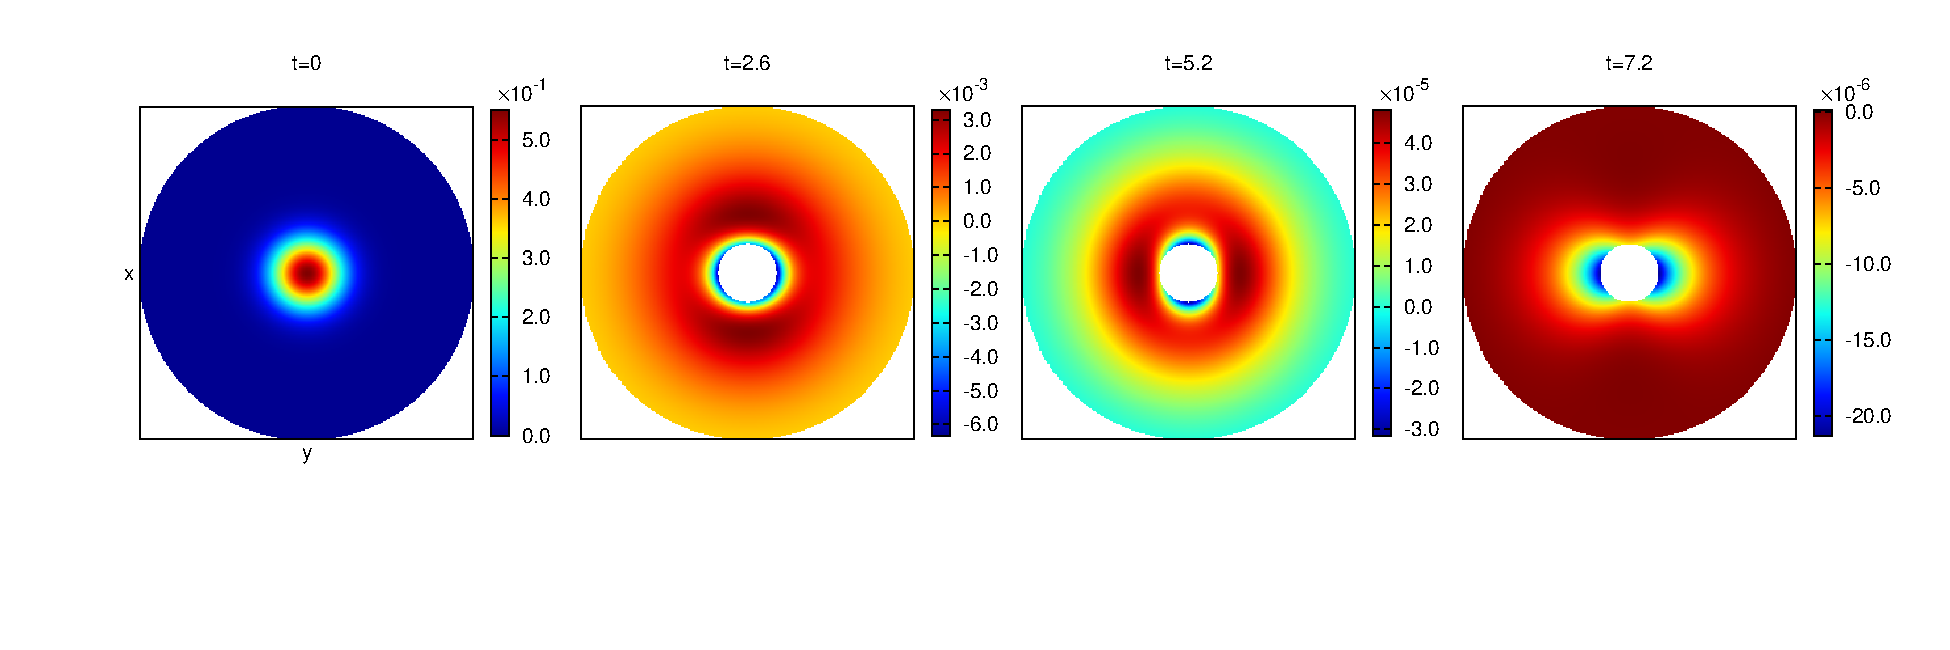
\includegraphics[width=7.0in,clip=true]{plots/bulkplots/L3/phi1/phi1_L3_snapshots_2.pdf}
\parbox{5.0in}{\caption{Snapshots of the scalar field on the $z=0$ slice.
        }\label{fig:snapshotsscalarfield-crop}}
\end{figure}

\begin{figure}[h]
        \centering
        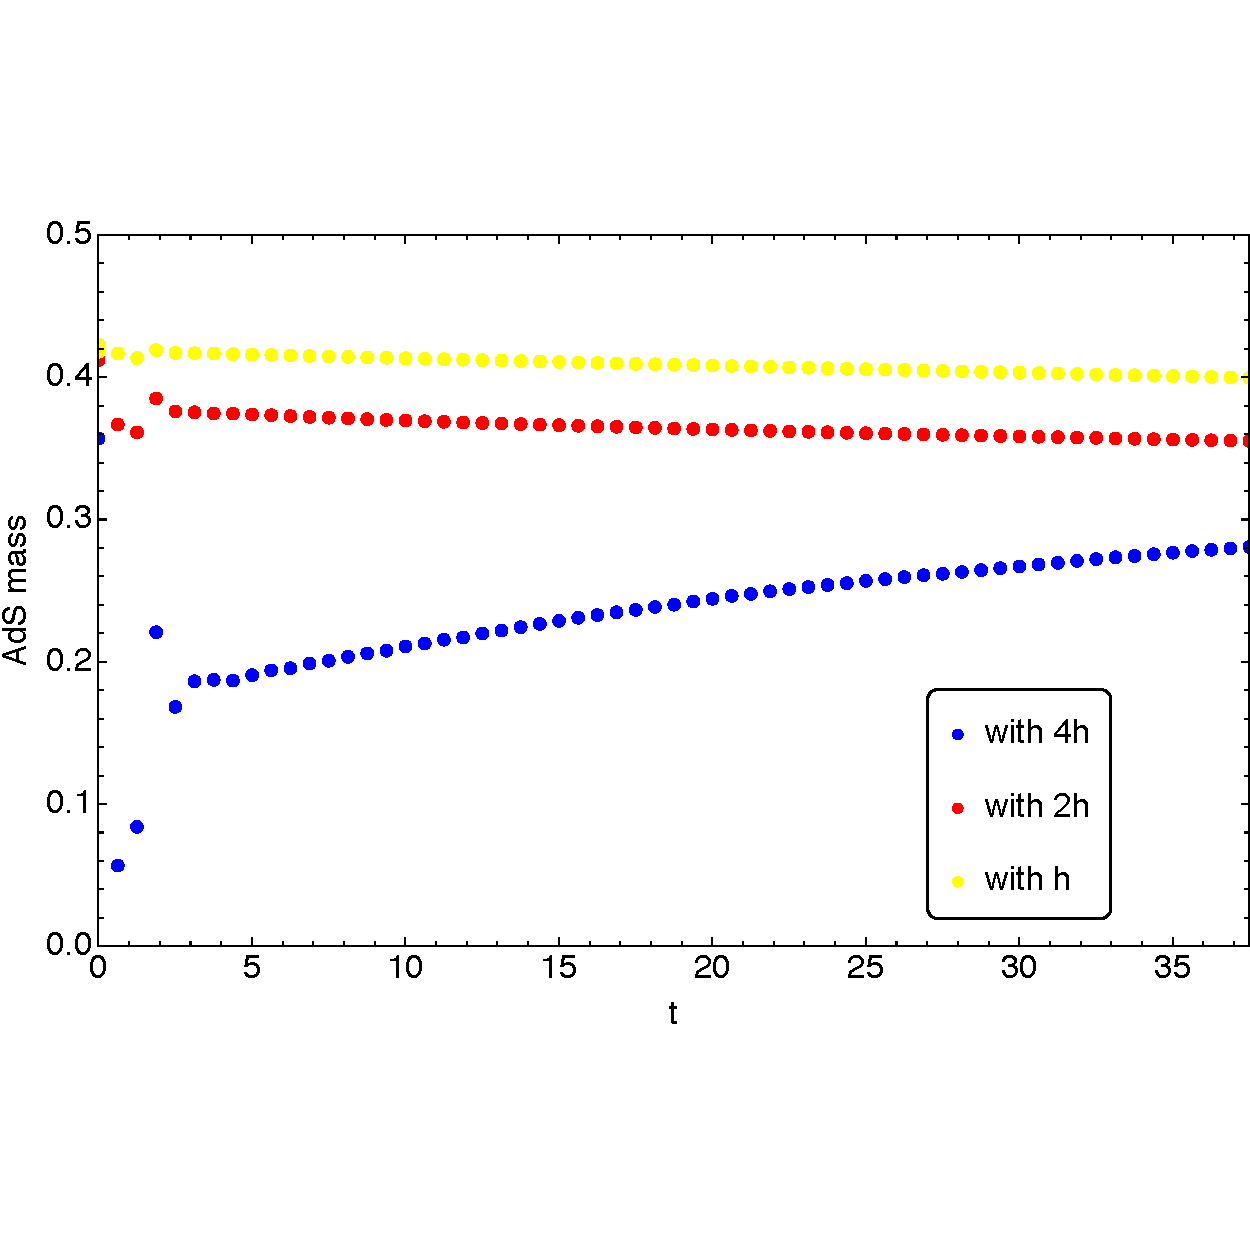
\includegraphics[width=4.0in,clip=true]{plots/timeseries/AdSmass/fullplotAdSmassL1L2L3res-cropped.pdf}
\parbox{5.0in}{\caption{Time series for AdS mass for different resolutions.
        }\label{fig:AdSmass-crop}}
\end{figure}

\begin{figure}[h]
        \centering
        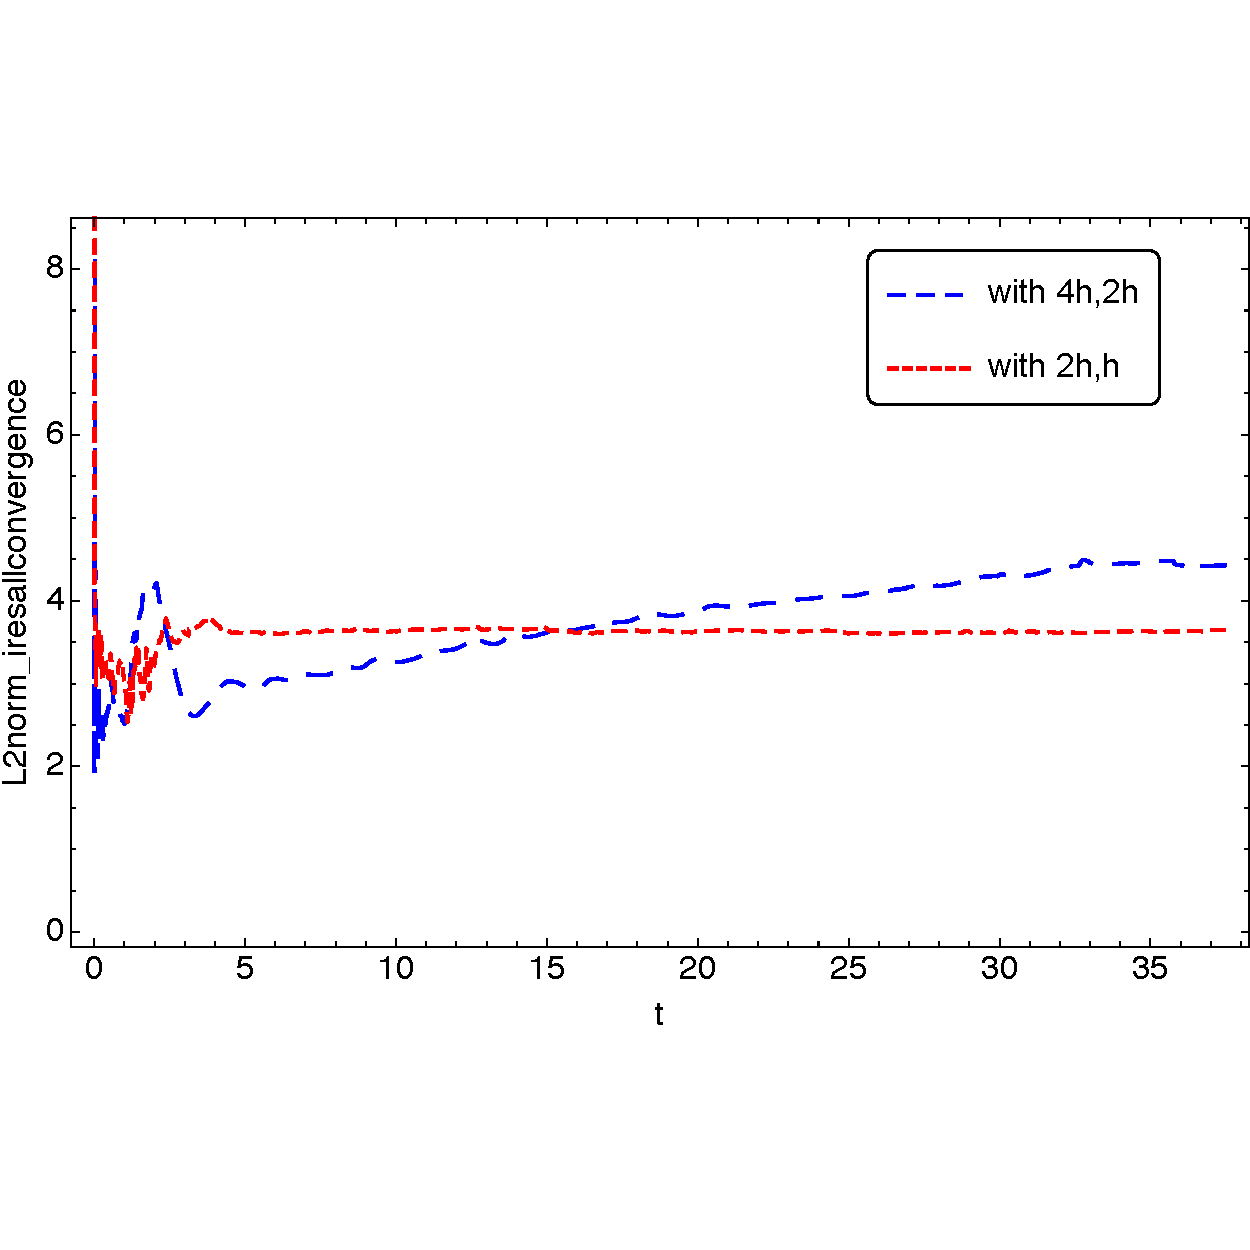
\includegraphics[width=4.0in,clip=true]{plots/timeseries/L2norm_iresallconvergence/fullplotiresallconvergenceL1L2L3res-cropped.pdf}
\parbox{5.0in}{\caption{Time evolution for $L^2$ norm of convergence factor for independent residual of EFE at different resolutions.
        }\label{fig:L2norm_iresallconvergence-crop}}
\end{figure}

\begin{figure}[h]
        \centering
        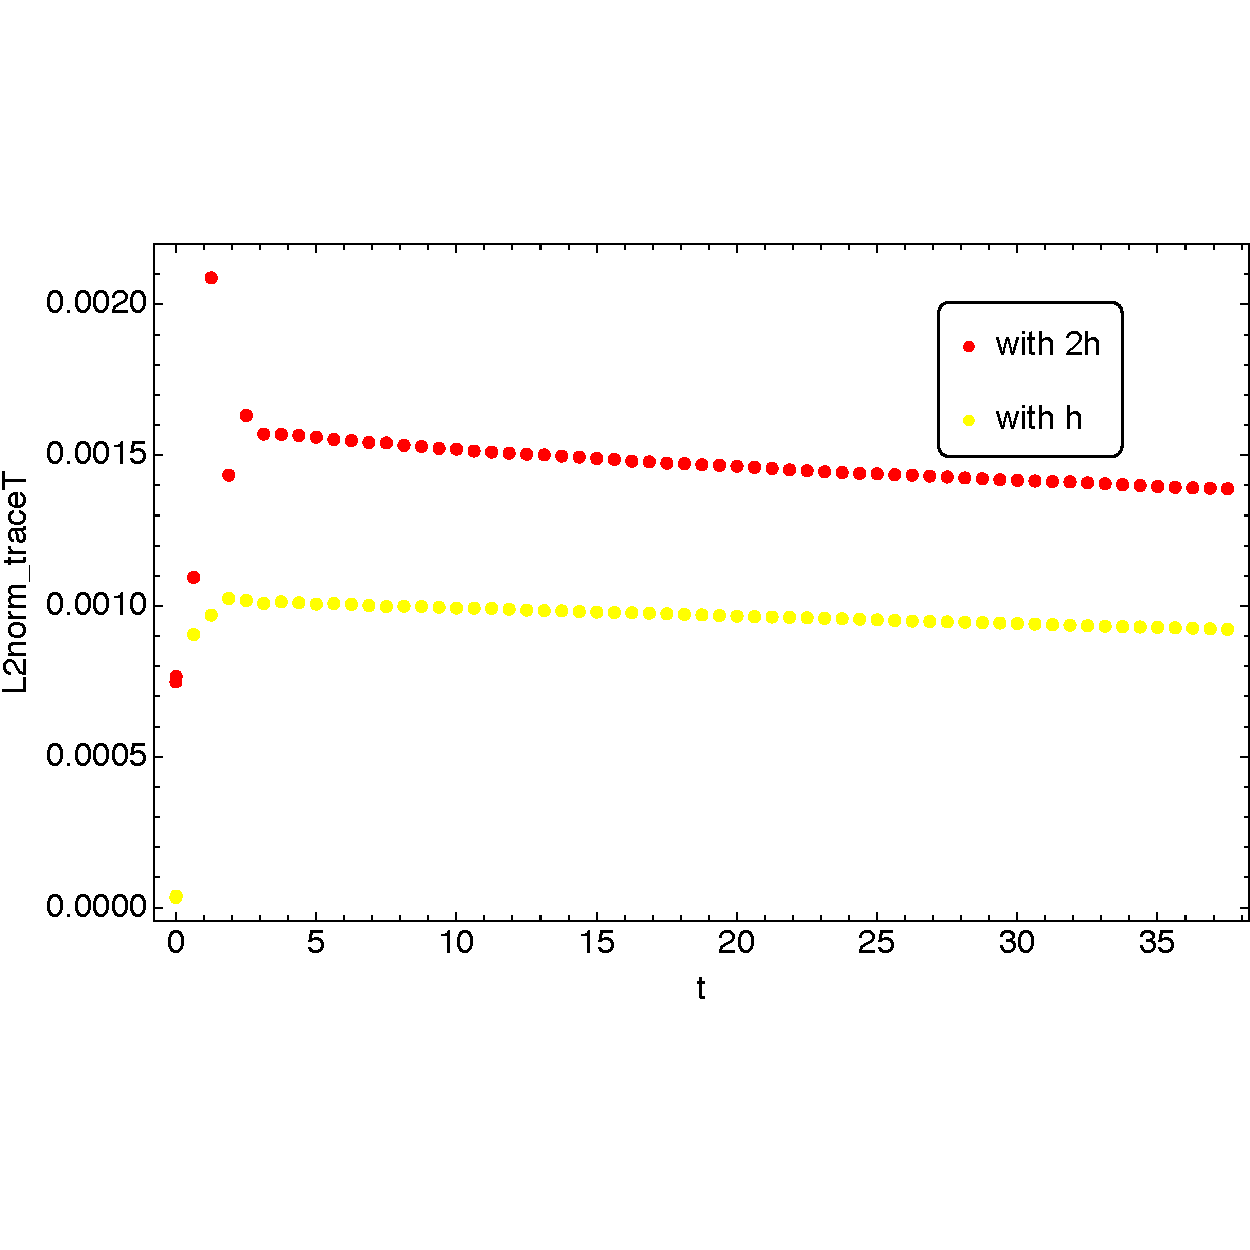
\includegraphics[width=4.0in,clip=true]{plots/timeseries/L2norm_quasiset_trace/fullplotL2normtraceL2L3res-cropped.pdf}
\parbox{5.0in}{\caption{Time evolution for $L^2$ norm of trace of quasi-local energy-momentum tensor of the boundary CFT at different resolutions.
        }\label{fig:L2norm_quasisettrace-crop}}
\end{figure}

\begin{figure}%
    \centering
    \subfloat[x-dependency]{{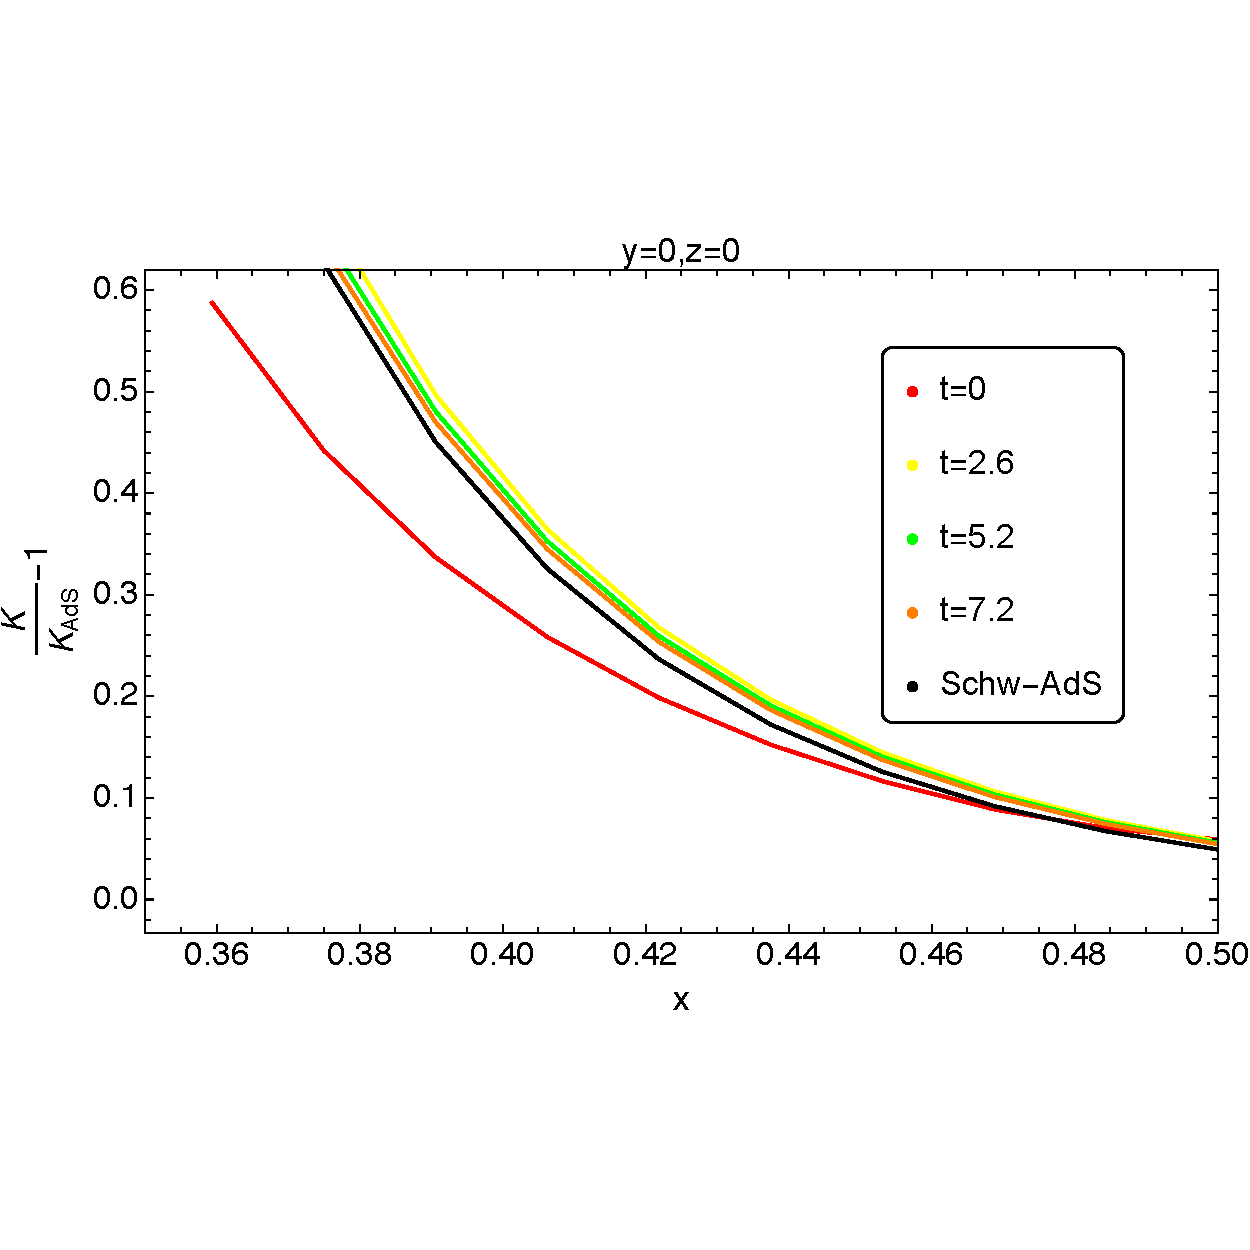
\includegraphics[width=3.0in]{/Users/lorenzorossi/Desktop/PhD/Research/Codes/lrossi_PAMR_AMRD_codes/Paper1/2019_3p1/plots/bulkplots/L2/relkretsch/fullplotxcoordrelkretschL2res-cropped.pdf} }}%
    \qquad
    \subfloat[y-dependency]{{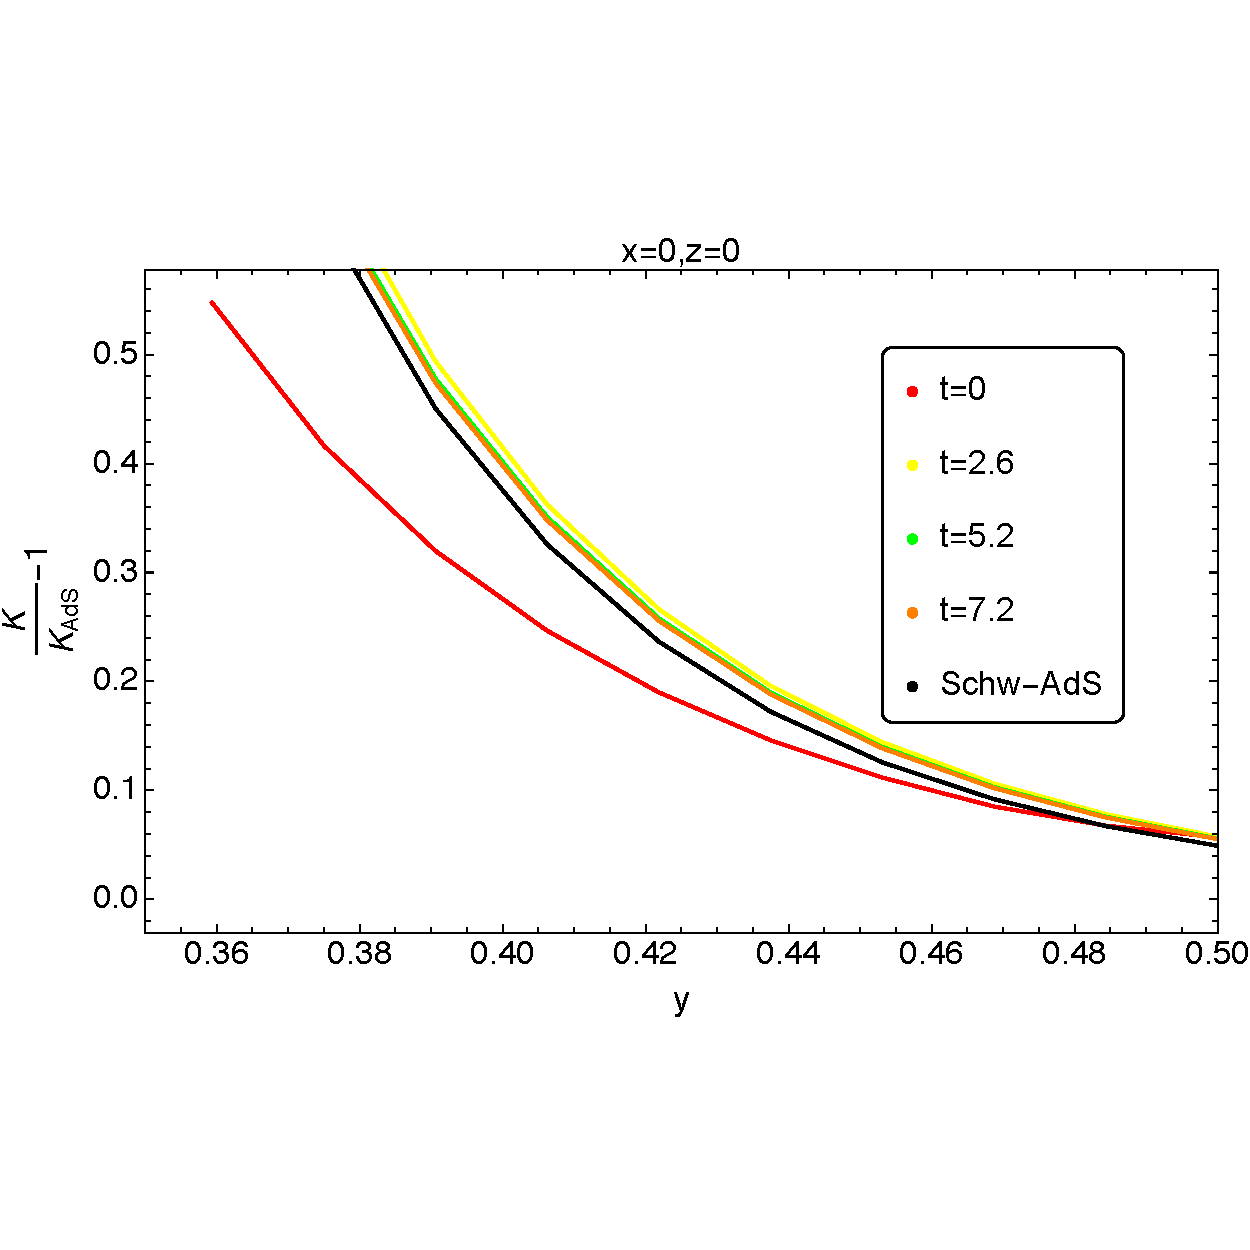
\includegraphics[width=3.0in]{/Users/lorenzorossi/Desktop/PhD/Research/Codes/lrossi_PAMR_AMRD_codes/Paper1/2019_3p1/plots/bulkplots/L2/relkretsch/fullplotycoordrelkretschL2res-cropped.pdf} }}%
    \caption{Time evolution of Kretschmann: the Kretschmann scalar of the solution approaches the one for Schwarzschild-AdS}%
    \label{fig:example}%
\end{figure}




\section{Discussion}\label{sec:Discussion}

\ack
Simulations were run on the {\bf Apocrita} cluster at Queen Mary University of London.

\appendix
\section{Generalized Harmonic Formulation}

The generalized harmonic formulation of the Einstein equations is based on coordinates $x^\mu$ that each satisfies a wave equation $\Box x^{\mu}=H^\mu$ with source functions $H^\mu$.
As long as the constraint $0=C^\mu \equiv H^\mu-\Box x^\mu$ is satisfied, we can then write the trace-reversed Einstein equations in $d$ dimensions with cosmological constant $\Lambda$
\begin{equation}
0=R_{\mu\nu} - \frac{2\Lambda}{d-2} g_{\mu\nu} - 8\pi\left( T_{\mu\nu} - \frac{1}{d-2} T g_{\mu\nu} \right)
\end{equation}
as
\begin{eqnarray}
0
&=& R_{\mu\nu} - \nabla_{(\mu} C_{\nu)} - \frac{2\Lambda}{d-2} g_{\mu\nu} - 8\pi\left( T_{\mu\nu} - \frac{1}{d-2} {T^\alpha}_\alpha g_{\mu\nu} \right) \nonumber \\
&=& R_{\mu\nu} - \nabla_{(\mu} H_{\nu)} + \nabla_{(\mu} \Box{x}_{\nu)} - \frac{2\Lambda}{d-2} g_{\mu\nu} - 8\pi\left( T_{\mu\nu} - \frac{1}{d-2} {T^\alpha}_\alpha g_{\mu\nu} \right) \nonumber \\
&=& -\frac{1}{2} g^{\alpha\beta} g_{\mu\nu,\alpha\beta} - g^{\alpha\beta}{}_{,(\mu}g_{\nu)\alpha,\beta} - H_{(\mu,\nu)} + H_\alpha \Gamma^\alpha{}_{\mu\nu} \nonumber \\
&&- \Gamma^\alpha{}_{\mu\beta}\Gamma^\beta{}_{\alpha\nu} - \frac{2\Lambda}{d-2} g_{\mu\nu} - 8\pi\left( T_{\mu\nu} - \frac{1}{d-2} {T^\alpha}_\alpha g_{\mu\nu} \right) \nonumber,
\end{eqnarray}
where the choice of $H_\mu = g_{\mu\nu} H^\nu$ constitutes a gauge choice. 
To suppress constraint-violating solutions that do not satisfy $C_\mu=0$, we supplement with constraint-damping terms as introduced in~\cite{Gundlach:2005eh} and obtain our final form of the Einstein equations
\begin{eqnarray}\label{eqn:efe_gh_modified}
&-& \frac{1}{2} g^{\alpha \beta} g_{\mu \nu, \alpha \beta} - 
{g^{\alpha \beta}}_{,(\mu} g_{\nu) \alpha, \beta} - H_{(\mu, \nu)} + H_\alpha {\Gamma^\alpha}_{\mu \nu} \nonumber \\
&-& {\Gamma^\alpha}_{\beta \mu} {\Gamma^\beta}_{\alpha \nu} - \kappa \left( 2 n_{(\mu} C_{\nu)} - (1+P) g_{\mu \nu} n^\alpha 
C_\alpha \right) \nonumber \\
&=&   \frac{2}{d-2} \Lambda g_{\mu \nu} + 8\pi \left( T_{\mu \nu} - 
\frac{1}{d-2} {T^\alpha}_\alpha g_{\mu \nu} \right).
\end{eqnarray}

\section{Convergence Tests}

Here we display a pair of numerical tests that demonstrate convergence trends for a representative simulation with no mesh refinement.
We do this for [pick simulation] with initial data parameters [display parameters]

To show that the solution we obtain is consistent, we compute the rate of convergence $Q(t,x,y,z)$ at each point on the grid with mesh spacing $\Delta$, for a given field $f_\Delta$
\begin{equation}\label{eq:qconv}
Q(t,x,y,z)=\frac{1}{\ln(2)}\ln\left( \frac{f_{4h}(t,x,y,z)-f_{2h}(t,x,y,z)}{f_{2h}(t,x,y,z)-f_{h}(t,x,y,z)} \right).
\end{equation}
We use second-order accurate finite difference stencils, and there is a factor of 2 between successive resolutions.
Thus, we expect $Q$ to asymptote to $Q=2$ in the limit $\Delta\rightarrow0$.

To show that the solution is converging to a solution of the Einstein equations, we compute an independent residual. 
This is obtained by taking the numerical solution and substituting it into a discretized version of
the Einstein equations, a component of which we denote $f_\Delta$. 
The independent residual should be purely numerical truncation error, so we can compute a convergence factor for it by using only two resolutions
\begin{equation}\label{eq:qires}
Q_{EFE}(t,x^i)=\frac{1}{\ln(2)}\ln\left( \frac{f_{2h}(t,x,y,z)}{f_{h}(t,x,y,z)} \right).
\end{equation}
Again, with second-order accurate finite difference stencils and with a factor of two between successive resolutions, we expect $Q$ to approach $Q=2$ as $\Delta\rightarrow0$.



%-------------------------------------------------------
% Bibliography
%-------------------------------------------------------
\section*{References}
\bibliographystyle{iopart-num}
\bibliography{3p1}



\end{document}

